%% LyX 2.3.5.2 created this file.  For more info, see http://www.lyx.org/.
%% Do not edit unless you really know what you are doing.
\documentclass[twocolumn,journal]{IEEEtran}
\usepackage[T1]{fontenc}
\usepackage[utf8]{inputenc}
\usepackage{float}
\usepackage{booktabs}
\usepackage{units}
\usepackage{url}
\usepackage{amsmath}
\usepackage{amsthm}
\usepackage{amssymb}
\usepackage{graphicx}
\usepackage[unicode=true,
 bookmarks=true,bookmarksnumbered=true,bookmarksopen=true,bookmarksopenlevel=1,
 breaklinks=false,pdfborder={0 0 0},pdfborderstyle={},backref=false,colorlinks=false]
 {hyperref}
\hypersetup{pdftitle={Your Title},
 pdfauthor={Your Name},
 pdfpagelayout=OneColumn, pdfnewwindow=true, pdfstartview=XYZ, plainpages=false}

\makeatletter

%%%%%%%%%%%%%%%%%%%%%%%%%%%%%% LyX specific LaTeX commands.
%% Because html converters don't know tabularnewline
\providecommand{\tabularnewline}{\\}
\floatstyle{ruled}
\newfloat{algorithm}{tbp}{loa}
\providecommand{\algorithmname}{Algorithm}
\floatname{algorithm}{\protect\algorithmname}

%%%%%%%%%%%%%%%%%%%%%%%%%%%%%% Textclass specific LaTeX commands.
% protect \markboth against an old bug reintroduced in babel >= 3.8g
\let\oldforeign@language\foreign@language
\DeclareRobustCommand{\foreign@language}[1]{%
  \lowercase{\oldforeign@language{#1}}}
\theoremstyle{plain}
\newtheorem{thm}{\protect\theoremname}
\theoremstyle{definition}
\newtheorem{defn}[thm]{\protect\definitionname}
\theoremstyle{definition}
\newtheorem{example}[thm]{\protect\examplename}
\theoremstyle{plain}
\newtheorem{cor}[thm]{\protect\corollaryname}
\theoremstyle{plain}
\newtheorem{rem}[thm]{\protect\remarkname}

%%%%%%%%%%%%%%%%%%%%%%%%%%%%%% User specified LaTeX commands.
% for subfigures/subtables
\usepackage[caption=false,font=footnotesize]{subfig}
\usepackage{algorithm,algorithmic}
\usepackage[bottom]{footmisc}

\makeatother

\providecommand{\corollaryname}{Corollary}
\providecommand{\definitionname}{Definition}
\providecommand{\examplename}{Example}
\providecommand{\remarkname}{Remark}
\providecommand{\theoremname}{Theorem}

\begin{document}
\title{Analysis of Polynomial Preconditioners}
\author{Ferdinand Vanmaele\\
Universität Heidelberg\\
Email: Vanmaele@stud.uni-heidelberg.de}
\markboth{Universität Heidelberg, ziti, Advanced Seminar}{Ferdinand Vanmaele}
\maketitle
\begin{abstract}
We explore solving large systems of linear equations using the GMRES
method, and study the effect of polynomial preconditiong for this
method. Besides improving convergence for difficult problems, polynomial
preconditioning allows us to reduce the amount of required scalar
products, at the cost of more SpMV (sparse matrix-vector multiplication)
operations. Preconditioning thus improves performance when solving
such systems on massively parallel systems, where communication costs
of scalar products can be a bottleneck.
\end{abstract}

\begin{IEEEkeywords}
Krylov subspaces, GMRES, polynomial preconditioning, communication-avoiding
\end{IEEEkeywords}


\IEEEpeerreviewmaketitle{}

\section{Introduction\label{sec:Introduction}}

Systems of linear equations $Ax=b$, where $A$ is a sparse matrix
of high dimension $n$, are widely solved in scientific computing
through iterative methods, that is, by finding a succession of approximations
from an initial value \cite[Chapter 6]{Magoules-2015}. This is in
contrast to direct methods, which are based on the initial factorization
of the coefficient matrix and give the result in a number of exactly
predictable operations. The disadvantage of direct methods lies in
a high number of arithmetic operations, and in the memory footprint
of storing matrices that were initially sparse \cite[Example 3.3]{Saad-2003}.

GMRES (Generalized Minimum Residual) method is an iterative method
suitable for a wide range of linear systems, including indefinite
and nonsymmetric systems. In every step, it minimizes the norm of
the residual vector $\|b-A\tilde{x}\|$ over a Krylov subspace. Constructing
the Krylov subspace is done through a Gram-Schmidt orthogonalization
procedure using inner products. On parallel and distributed systems,
computing inner products requires global reduction operations involving
all processes. In comparison, sparse matrix-vector multiplications
only need to exchange data between neighbors \cite[14.5]{Magoules-2015}.

To address this issue, we consider preconditioned systems $M^{-1}Ax=M^{-1}b$,
where $M^{-1}$ is a (typically low degree) matrix polynomial. This
preconditioned system has the same solution as the original system
$Ax=b$, but may achieve faster convergence. Achieving a certain tolerance
for the residual thus occurs in less GMRES steps (inner products),
at the expense of more matrix-vector multiplications in every step.
We discuss a polynomial which does not require knowledge of the spectrum
of the matrix $A$. Finding the coefficients of $M^{-1}$ requires
a (possibly dense) matrix-matrix multiplication. This cost can be
controlled by the degree of the polynomial, depending on the difficulty
of the problem, making it more granular than classical preconditioners
such as Incomplete LU (ILU) factorizations. 

\section{Related Work\label{sec:Related-Work}}

Saad \cite{Saad-1986} introduced the GMRES method for systems in
which the coefficent matrix $A$ is nonsymmetric or indefinite. Indefinite
systems commonly arise, for example, in mixed finite element methods
for solving problems in fluid and solid mechanics \cite{Benzi-2005,Rozlo=00017En=0000EDk-2018}.

Since then, the algorithms have been included in general textbooks
on numerical linear algebra and scientific computing \cite{Saad-2003,Trefethen-1997,Magoules-2015}.
Implementations are available in MATLAB and scientific computing libraries
such as GSL and TRILINOS. Liu \cite{Liu-2015} discusses polynomial
preconditioning with GMRES and introduces a way to find the coefficients
without knowledge of the matrix spectrum. Loe et. al. \cite{Loe-2019}
conducted further experiments on (shared-memory) parallel hardware
with TRILINOS. 

Besides polynomial preconditioning, Block Krylov methods also help
reduce the effect of inner products on communication. Saad \cite[6.12]{Saad-2003}
put forward an overview and gives further references. 

After revisiting theoretical results on Krylov subspaces and GMRES
in Sections \ref{sec:Krylov-subspaces}, \ref{sec:The-GMRES-method}
and \ref{sec:Convergence-of-GMRES}, we introduce polynomial preconditioning
and its advantages in Section \ref{sec:Preconditioning}. In Section
\ref{sec:Numerical-experiments} we test the impact of polynomial
preconditioning on convergence for several test problems. 

\section{Krylov subspaces\label{sec:Krylov-subspaces} }

We will look at iterative methods for solving the linear system $Ax=b$
of dimension $n$, where $A$ is an invertible square matrix, with
approximate solutions in Krylov subspaces. These methods can be applied
to either real or complex matrices. We introduce Krylov subspaces
and construct an orthonormal basis. Solving a least squares problem
to find the minimum residual for vectors in this subspace leads to
the GMRES method. 
\begin{defn}[{\cite[6.2]{Saad-2003}}]
The \textbf{Krylov subspace} of order $m$, denoted by $\mathcal{K}_{p}$,
is the vector space spanned by $v\in\mathbb{R}^{n}$ and the first
$m-1$ powers of $A$:
\[
\mathcal{K}_{m}(A,v)=\text{span}\{v,Av,A^{2}v,\ldots,A^{m-1}v\}.
\]
The Krylov subspaces form an increasing family of subspaces, with
dimension bounded by $n$. It is the subspace of all vectors in $\mathbb{R}^{n}$
which can be written as $x=p(A)v$, where $p$ is a polynomial of
degree not exceeding $m-1$.  
\end{defn}
In practice, constructing the Krylov subspaces amounts to determining
their basis. The power basis $(v,Av,A^{2}v,\ldots,A^{m-1}v)$ converges
to (a multiple of) an eigenvector that corresponds to the largest
eigenvalue of $A$, in absolute value \cite[10.2]{Magoules-2015}.
Therefore we construct an orthonormal basis $\{v_{1},v_{2},\ldots,v_{m}\}$
as follows. 

\textbf{Arnoldi's method} applies the (modified) Gram-Schmidt orthonormalization
procedure to the vectors obtained by successive products of the matrix
$A$. Algorithm \ref{alg:Arnoldi-Modified-Gram-Schmidt} \cite[6.3.2]{Saad-2003}
gives a practical implementation. 

\begin{algorithm}[h]
Choose a vector $v_{1}$ of norm 1

\textbf{For} $j=1,2,\ldots,m$ \textbf{Do}:

\hspace{2em}Compute $w_{j}:=Av_{j}$

\hspace{2em}\textbf{For} $i=1,\cdots,j$ \textbf{Do}:

\hspace{2em}\hspace{2em}$h_{ij}=(w_{j},v_{i})$

\hspace{2em}\hspace{2em}$w_{j}:=w_{j}-h_{ij}v_{i}$

\hspace{2em}\textbf{EndDo}

\hspace{2em}$h_{j+1,j}=\|w_{j}\|_{2}$. If $h_{j+1,j}=0$ \textbf{Stop}

\hspace{2em}$v_{j+1}=w_{j}/h_{j+1,j}$

\textbf{EndDo}

\caption{Arnoldi-Modified Gram-Schmidt\label{alg:Arnoldi-Modified-Gram-Schmidt}}
\end{algorithm}

The modified Gram-Schmidt procedure has better numerical properties
than the classical procedure \cite[6.3.2]{Saad-2003}, but requires
additional synchronization points when implemented on a parallel computer.
Additional methods such as DCGS2 were introduced to address these
issues \cite{Hernandez-2005}. Householder transformations, which
are relatively costly but stable, were also proposed \cite[2.3.4]{Barret-1994}.

The following important relations hold for the Arnoldi basis: 
\[
AV_{m}=V_{m+1}\overline{H}_{m},\qquad V_{m}^{T}AV_{m}=H_{m},
\]
where $V_{m}$ denotes the $n\times m$ matrix with orthonormal column
vectors $v_{1},\ldots,v_{m}$, $\overline{H}_{m}$ the $(m+1)\times m$
Hessenberg matrix with nonzero entries $h_{ij}$, and $H_{m}$ the
matrix obtained from $\overline{H}_{m}$ by deleting its last row:
\cite[Proposition 6.5]{Saad-2003}
\[
H_{m}=\begin{pmatrix}h_{1,1} & h_{1,2} & \cdots & \cdots & h_{1,m}\\
h_{2,1} & h_{2,2} &  &  & \vdots\\
 & h_{3,2} & \ddots &  & \vdots\\
 &  & \ddots & \ddots & \vdots\\
 &  &  & h_{m,m-1} & h_{m,m}
\end{pmatrix}.
\]


\section{The GMRES method\label{sec:The-GMRES-method}}

Let $r_{0}=b-Ax_{0}$ denote the residual for an initial approximation
$x_{0}$. Let $\mathcal{K}_{m}:=\mathcal{K}_{m}(A,r_{0})$. We seek
to minimize the residual on the affine subspace $x_{0}+\mathcal{K}_{m}$
of dimension $m$. 
\begin{defn}
Choose $v_{1}=r_{0}/\|r_{0}\|$ for the Arnoldi basis, and let $\beta:=\|r_{0}\|$.
Any vector in $x_{0}+\mathcal{K}_{m}$ can be written as $x=x_{0}+V_{m}y$,
where $y\in\mathbb{R}^{m}$. By the above relation, the objective
is given as: \cite[6.5.1]{Saad-2003}
\begin{align*}
J(y) & =\|b-A(x_{0}+V_{m}y)\|_{2}=\|r_{0}-AV_{m}y\|_{2}\\
 & =\|\beta v_{1}-V_{m+1}\overline{H}_{m}y\|_{2}.
\end{align*}
By orthonormality of $V_{m+1}$ column vectors, $J(y)=\|\beta e_{1}-\overline{H}_{m}y\|$.
The \textbf{GMRES approximation} is then the unique vector  of $x_{0}+\mathcal{K}_{m}$
which minimizes $J$.  
\end{defn}
This results in Algorithm \ref{alg:GMRES} (\cite[Algorithm 6.9]{Saad-2003}).

\begin{algorithm}[h]
Compute $r_{0}=b-Ax_{0}$, $\beta:=\|r_{0}\|_{2}$, and $v_{1}:=r_{0}/\beta$

\textbf{For} $j=1,2,\ldots,m$ \textbf{Do}:

\hspace{2em}$\langle$ step $n$ of Arnoldi iteration, Algorithm
\ref{alg:Arnoldi-Modified-Gram-Schmidt} $\rangle$

\textbf{EndDo}

Define the $(m+1)\times m$ Hessenberg matrix $\overline{H}_{m}=\{h_{ij}\}_{1\leq i\leq m+1,1\leq j\leq m}$

Compute $y_{m}$ the minimizer of $\|\beta e_{1}-\overline{H}_{m}y\|_{2}$
and $x_{m}=x_{0}+V_{m}y_{m}$\caption{GMRES\label{alg:GMRES}}
\end{algorithm}

Computing $y_{m}$ is an $(m+1)\times m$ matrix least squares problem
with Hessenberg structure that can be solved via QR factorization
in the usual manner, at the cost of $\mathcal{O}(m^{2})$ operations.
To save further work, rather than construct QR factorizations of the
successive matrices $\overline{H}_{1},\overline{H}_{2},\ldots$ independently,
we can use an updating process to get the QR factorization of $\overline{H}_{m}$
from that of $\overline{H}_{m-1}$. Doing so requires a single \textbf{Givens
rotation} and $\mathcal{O}(m)$ work \cite[Mechanics of GMRES]{Trefethen-1997}.

This approach also enables obtaining the residual norm of the approximate
solution without computing $x_{k}$, thus allowing to decide when
to stop the algorithm inexpensively \cite[3.2]{Saad-1986}. Saad \cite{Saad-1986,Saad-2003}
gives the detailed implementation.

Consider now the algorithm from a practical viewpoint. As $m$ increases,
the computational cost increases at least as $\mathcal{O}(m^{2}n)$
because of the Gram-Schmidt orthogonalization. The memory cost increases
as $\mathcal{O}(mn)$. For large $n$ this limits the largest value
of $m$ that can be used. One remedy is to restart the algorithm periodically
\cite[6.4.1, 6.5.5]{Saad-2003}. This is the \textbf{restarted GMRES}
or GMRES(m) algorithm. Note that GMRES(m) does not necessarily converge,
unless the matrix $A$ is positive definite \cite[3.4]{Saad-1986}.

\section{Convergence of GMRES\label{sec:Convergence-of-GMRES}}

Because $\|r_{m}\|$ is as small as possible for the subspace $\mathcal{K}_{m}$,
by enlarging $\mathcal{K}_{m}$ to the space $\mathcal{K}_{m+1}$
we can only decrease the residual norm, or at worst leave it unchanged.
Thus we observe that GMRES converges monotonically: $\|r_{m+1}\|\leq\|r_{m}\|$.
After $n$ steps (for an $n\times n$ problem), we have $\mathcal{K}_{n}=\mathbb{C}^{n}$
and the full GMRES algorithm is guaranteed to converge. However, for
GMRES to be useful, it must converge to satisfactory precision in
$n\ll m$ steps \cite[p.270]{Trefethen-1997}.

To obtain more useful information about convergence, we must turn
to the following problem. The iterate $x_{m}\in x_{0}+\mathcal{K}_{m}$
can be written as $x_{m}=x_{0}+q(A)r_{0}$, where $q$ is a polynomial
of degree $m-1$. 

Furthermore, as $x_{m}$ minimizes $\|r_{m}\|=\|b-Ax_{m}\|$ in the
affine subspace $x_{0}+\mathcal{K}_{m}$, we have $x_{m}=x_{0}+q_{m}(A)r_{0}$,
where $q_{m}$ is the polynomial that solves: \cite[Lemma 6.31]{Saad-2003}
\begin{align*}
\|r_{m}\| & =\|b-A(x_{0}+q_{m}(A)r_{0})\|=\min_{q\in P_{m-1}}\|(I-Aq(A))r_{0}\|\\
 & =\min_{p\in P_{m},p(0)=1}\|p(A)r_{0}\|.
\end{align*}

The polynomial $p$ is determined by GMRES. We can show:
\begin{thm}[{\cite[Proposition 6.32]{Saad-2003} }]
Suppose $A$ is diagonalizable, satisfying $A=X\Lambda X^{-1}$ with
$\Lambda=\text{diag}\{\lambda_{1},\lambda_{2},\ldots,\lambda_{n}\}$
is the diagonal matrix of eigenvalues. We have the following upper
bound on the residual:
\[
\|r_{m}\|\leq\kappa_{2}(X)\,\min_{p\in\mathbb{P}_{m},p(0)=1}\max|p(\lambda_{i})|.
\]
\end{thm}
This theorem can be summarized in words as follows. If $A$ is not
too far from normal in the sense that $\mathcal{K}(X)$ is not too
large, and if properly normalized degree $m$ polynomials can be found
whose size on the spectrum $\Lambda(A)$ decreases quickly with $m$,
then GMRES converges quickly \cite[p.271]{Trefethen-1997}.
\begin{example}
Let $n=4000$, with entries sampled from $\mathcal{N}(2,0.5/\sqrt{n})$.
The eigenvalues are roughly uniformly distributed in the disk of radius
$\frac{1}{2}$ centered at $z=2$. $\|p(A)\|$ is then approximately
minimized by $p(z)=(1-z/2)^{m}$, with a convergence rate of $4^{-m}$
\cite{Trefethen-1997}.
\end{example}
\begin{cor}[\cite{Saad-1986}]
Suppose $A$ is positive real with symmetric part $M=\frac{1}{2}(A+A^{T})$.
We have the following upper bound on the residual:
\[
\|r_{m}\|\leq\left(1-\frac{\lambda_{\min}(1/2(A^{T}+A))^{2}}{\lambda_{\max}(A^{T}A)}\right)^{\nicefrac{m}{2}}\|r_{0}\|.
\]
\end{cor}
In particular, if $A$ is symmetric positive definite, we have:
\[
\|r_{m}\|\leq\left(\frac{\kappa(A)^{2}-1}{\kappa(A)^{2}}\right)^{\nicefrac{m}{2}}\|r_{0}\|,
\]
where $\kappa=\|A\|\|A^{-1}\|$ denotes the condition number of $A$.


\section{Preconditioning\label{sec:Preconditioning}}

For any nonsingular $n\times n$ matrix $M$, the system 
\[
M^{-1}Ax=M^{-1}b
\]
 has the same solution as the nonsingular system $Ax=b$. Solving
this system depends on the properties of $M^{-1}A$, and may require
fewer steps to converge than the original system \cite[10.1]{Saad-2003}.
We call $M$ the \textbf{preconditioner}. The preconditioner can be
either applied to the left or right. Latter leads to the system
\begin{align*}
AM^{-1}u & =b,\\
x & =M^{-1}u.
\end{align*}
This amounts to making the change of variables $u=Mx$, and solving
the system with respect to the unknown $u$ \cite[9.1]{Saad-2003}. 

$M$ should meet the following requirements:
\begin{itemize}
\item $M$ lies between $M=A$ (for the equally hard to solve system $x=A^{-1}b$)
and $M=I$ (for the original system $Ax=b)$.
\item $M^{-1}$ is inexpensive to apply to an arbitrary vector.
\item $M$ is ``close enough'' to $A$, in the sense that the preconditioned
system $M^{-1}Ax=M^{-1}b$ converges more quickly than the system
$Ax=b$. Specifically, we want $\|I-M^{-1}A\|$ to be small and the
eigenvalues of $M^{-1}A$ close to 1, or clustered around some other
value \cite[Lecture 40]{Trefethen-1997}. 
\end{itemize}
Note the following differences when preconditioning GMRES: \cite[9.3]{Saad-2003}\medskip{}

\begin{itemize}
\item Left preconditioning:
\begin{itemize}
\item builds an orthogonal basis of the Krylov subspace 
\[
\text{span}\{r_{0},M^{-1}Ar_{0},\dots,(M^{-1}A)^{m-1}r_{0}\};
\]
\item obtains the residuals relative to the preconditioned system, i.e.
$M^{-1}(b-Ax_{m})$;
\item uses one preconditioning operation at the beginning of the outer loop,
$r_{0}=M^{-1}(b-Ax_{0}$).
\end{itemize}
\item Right preconditioning:
\begin{itemize}
\item builds an orthogonal basis of the Krylov subspace 
\[
\text{span}\{r_{0},AM^{-1}r_{0},\dots,(AM^{-1})^{m-1}r_{0}\};
\]
\item obtains the residuals relative to the initial system, i.e. $b-Ax_{m}$;
\item uses one preconditioning operation at the end of the outer loop, $x_{m}=x_{0}+M^{-1}V_{m}y_{m}$.
\end{itemize}
\end{itemize}

\subsection{Polynomial preconditioning}

Consider the characteristic polynomial $\chi_{A}$ of $A$. With the
Caley-Hamilton theorem, we have 
\[
\chi_{A}(A)=a_{n}A^{n}+a_{n-1}A^{n-1}+\cdots+a_{1}A+a_{0}I=0,
\]
and so, for $a_{0}\neq0$, 
\[
A^{-1}=\frac{1}{a_{0}}(-a_{n}A^{n-1}-a_{n-1}A^{n-2}-\cdots-a_{1}I).
\]
It thus makes sense to approximate $A^{-1}$ with a polynomial $s(A)$.
We set $M^{-1}=s(A)$, and assume $s$ to have degree $d\ll n$. Note
that $s(A)A=As(A)$, so left and right preconditioning build the same
Krylov subspace. We call $M^{-1}$ a \textbf{polynomial preconditioner}.

The matrix $s(A)$ does not need to be formed explicitly: $s(A)v$
can be computed for any vector $v$ from a sequence of matrix-by-vector
products \cite[12.3]{Saad-2003}. In particular, \textbf{Horner's
method} computes $s(A)v$ with $d$ matrix-vector products: 
\begin{align*}
s(A)v & =s_{d+1}A^{d}v+s_{d}A^{d-1}v+\cdots+s_{1}v\\
 & =A(A\cdots(s_{d+1}Av+s_{d}v)+\cdots+s_{2}v)+s_{1}v.
\end{align*}

\begin{rem}
A polynomial preconditioner may be combined with other preconditioners
$M'$, such as ILU($k$), by solving the system:
\[
s(M'^{-1}A)M'^{-1}A=s(M'^{-1}A)M'^{-1}b.
\]
\end{rem}
We now compute a polynomial preconditioner related to the GMRES polynomial,
corresponding to a minimal residual $\|p(A)r_{0}\|=\|(I-Aq(A))r_{0}\|$.
For a preconditioner, we compute $q(A)$ instead. Denote this polynomial
by $M^{-1}=s(A)$ as above, and let $v_{0}\neq0$. We solve:
\[
\min\|(I-M^{-1}A)v_{0}\|=\min_{q\in\mathbb{P}_{d}}\|v_{0}-Aq(A)v_{0}\|
\]
by building a power basis $Y=\{v_{0},Av_{0},\ldots,A^{d}v_{0}\}$,
and solving the normal equations 
\[
(AY)^{T}AYy=(AY)v_{0}.
\]

The elements of $y$ are the coefficients of $M^{-1}$. Note the
following:
\begin{itemize}
\item The method requires no knowledge of the spectrum of $A$, unlike Chebyshev
or least squares polynomials \cite{Liu-2015}.
\item The method becomes unstable as the columns of $Y$ lose linear independence,
but its results are generally sufficient for low-degree (up to $d=10$)
polynomials \cite{Liu-2015}.
\item The coefficients of the polynomial depend on the choice of $v_{0}$.
Using a randomly chosen vector may be preferable in this case \cite{Loe-2019}.
\item The matrix $AY$ is a matrix of dimension $n\times(d+1)$, and takes
$d+1$ matrix-vector products to compute. The product $(AY)^{T}AY$
is of dimension $(d+1)\times(d+1)$ and requires a matrix-matrix multiplication.
With $d\ll n$, the system $(AY)^{T}AYy=(AY)v_{0}$ is of small dimension
and can be solved with a direct method such as LU decomposition. 
\end{itemize}

\section{Numerical experiments\label{sec:Numerical-experiments}}

For every problem, the right-hand side is sampled from $\mathcal{N}(0,1)$,
the real normal distribution of mean $0$ and standard deviation 1.
Orthonormalization was done using the Modified Gram-Schmidt procedure.
Right preconditioned GMRES is used for comparing residuals $\|b-Ax_{i}\|$
between the initial and preconditioned systems. The vector $v_{0}$
for computing the power basis $Y$ is sampled from $U[-1,1]$, the
uniform distribution on the interval $[-1,1]$. 

Some of the problems considered are very difficult for GMRES to solve,
and, considering the small dimension $n$, may be better suited for
direct solvers. They nonetheless give a good indication of the difficulties
involved when using GMRES.
\begin{enumerate}
\item \label{enu:problem-1}The \textbf{Circle Eigenvalue Matrix} of size
$n=2000$, a block diagonal matrix with $2\times2$ blocks:
\[
\begin{pmatrix}1+\cos(\alpha) & \sin(\alpha)\\
-\sin(\alpha) & 1+\cos(\alpha)
\end{pmatrix},
\]
$\alpha\in2k\frac{\pi}{n},\ k\in\{0,2,\ldots,n-2\}$. All eigenvalues
of this matrix are on the unit circle on the complex plane with center
$(1,0)$ \cite{Liu-2015}. The condition number is estimated at $6.3662\times10^{3}$.
\item \label{enu:problem-2}The \textbf{Bidiagonal Matrix} of size $n=5000$
with diagonal elements 0.1, 0.2, 0.3, $\ldots,$ 0.9, 1, 2, 3, $\ldots,$
4990, 4991 (\emph{BiDiag1}). The superdiagonal elements are all set
to 0.2 \cite{Liu-2015}. The symmetric part is positive definite,
and the condition number estimated at $8.4589\times10^{4}$.  
\item \label{enu:problem-3}As problem \ref{enu:problem-2}, but the diagonal
elements are set to 10, 11, 12, $\ldots,$ 5009 (\emph{BiDiag2}).
The condition number is estimated at $5.0137\times10^{3}$. 
\item \label{enu:problem-4}\textbf{S1RMQ4M1} (Matrix Market), a real symmetric
positive definite matrix of size $n=5489$. The matrix has high condition
number, estimated at $3.21\times10^{6}$ by Matrix Market.
\item \label{enu:problem-5}\textbf{E20R0100} (Matrix Market), a real non-symmetric
indefinite matrix of size $n=4241$. The matrix has high condition
number, estimated at $2.15\times10^{10}$ by Matrix Market. This matrix
serves as a counter-example for classical preconditioners such as
ILU, where their application may result in a worse condition number. 
\item \label{enu:problem-6}\textbf{SHERMAN5} (Matrix Market), a real non-symmetric
matrix of size $n=3312$. The condition number is estimated at $3.9\times10^{5}$
by Matrix Market. This matrix serves as an example where polynomial
preconditioning can worsen convergence.
\end{enumerate}
Polynomials of degree 3, 5, 7, and 10 are used for most problems.
Implementation was done in MATLAB\footnote{See \url{https://github.com/fvanmaele/polynomial-preconditioning}
for the implementation and supplementary materials.}, based on \texttt{gmres.m} from the Netlib Repository.

\subsection{Numerical properties}

As explained in Section \ref{sec:Preconditioning}, we expect a preconditioner
to be effective if the eigenvalues of $M^{-1}A$ are clustered around
a constant value, such as 1. For most test problems, after applying
the polynomial preconditioner this was indeed the case. The results
are summarized in Table \ref{tab:spectra-stats}. The spectrum of
E20R0100 after applying a degree 10 polynomial is shown in Fig. \ref{fig:spec_e20r0100}. 

For the symmetric positive definite matrix S1RMQ4M1, preconditioning
with degree 7 and degree 9 polynomials lead to negative eigenvalues.
These eigenvalues were outliers, and the behavior was not observed
for polynomials of a different degree. One may however expect that
$M^{-1}A$, while symmetric, is not positive definite in general.
This limits the use of the preconditioner with the Preconditioned
CG method \cite{Saad-1985}, which depends on a symmetric positive
definite preconditioner.

\begin{table}[b]
\caption{Extreme values, mean $\mu$, and standard deviation $\sigma$ for
$|\lambda(A)|$, the (magnitude of the) spectrum of $A$.\label{tab:spectra-stats}}
\medskip{}

\centering{}%
\begin{tabular}{|c|c|l|l|l|l|}
\hline 
{\scriptsize{}Matrix $A$} & {\scriptsize{}$\deg$} & {\scriptsize{}$\min(|\lambda(A)|)$} & {\scriptsize{}$\max(|\lambda(A)|$} & {\scriptsize{}$\mu(|\lambda(A)|$} & {\scriptsize{}$\sigma(|\lambda(A)|)$}\tabularnewline
\hline 
\hline 
{\scriptsize{}CEM} & {\scriptsize{}–} & {\scriptsize{}0.00314} & {\scriptsize{}2} & {\scriptsize{}1.2742} & {\scriptsize{}0.61523}\tabularnewline
\hline 
{\scriptsize{}CEM} & {\scriptsize{}10} & {\scriptsize{}0.01727} & {\scriptsize{}1.2070} & {\scriptsize{}0.94540} & {\scriptsize{}0.14954}\tabularnewline
\hline 
{\scriptsize{}BiDiag1} & {\scriptsize{}–} & {\scriptsize{}0.1} & {\scriptsize{}4991} & {\scriptsize{}2491.5} & {\scriptsize{}1443.5}\tabularnewline
\hline 
{\scriptsize{}BiDiag1} & {\scriptsize{}3} & {\scriptsize{}0.00024} & {\scriptsize{}1.1509} & {\scriptsize{}0.95895} & {\scriptsize{}0.19989}\tabularnewline
\hline 
{\scriptsize{}S1RMQ4M1} & {\scriptsize{}–} & {\scriptsize{}0.37970} & {\scriptsize{}6.8743e+05} & {\scriptsize{}8.6760e+04} & {\scriptsize{}1.2595e+05}\tabularnewline
\hline 
{\scriptsize{}S1RMQ4M1} & {\scriptsize{}3} & {\scriptsize{}7.7127e-06} & {\scriptsize{}1.2028} & {\scriptsize{}0.47948} & {\scriptsize{}0.49665}\tabularnewline
\hline 
{\scriptsize{}E20R0100} & {\scriptsize{}–} & {\scriptsize{}1.3999e-06} & {\scriptsize{}13.057} & {\scriptsize{}4.3537} & {\scriptsize{}4.0740}\tabularnewline
\hline 
{\scriptsize{}E20R0100} & {\scriptsize{}10} & {\scriptsize{}4.8582e-06} & {\scriptsize{}1.0902} & {\scriptsize{}0.71268} & {\scriptsize{}0.44947}\tabularnewline
\hline 
\end{tabular}
\end{table}

\begin{figure}[t]
\begin{centering}
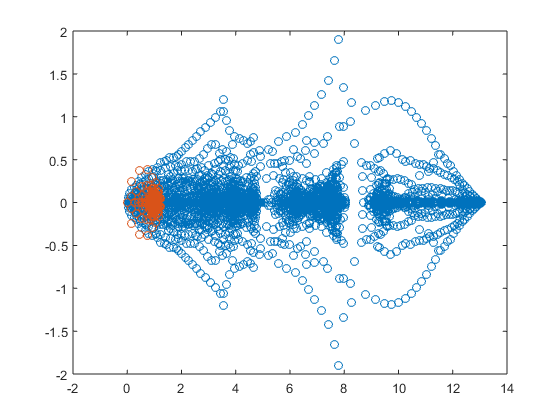
\includegraphics[width=0.45\textwidth]{example_5_spec}
\par\end{centering}
\caption{Spectrum of $A$ (blue) and $M^{-1}A$ (orange, $d=10$) for E20R0100\label{fig:spec_e20r0100}}
\end{figure}

For most test problems, the condition number was inversely proportional
to the degree of the applied polynomial. In those cases, a degree
$10$ polynomials decreased the condition number by a degree of magnitude.
The exception was SHERMAN5, where the condition number varied strongly
for different degree polyomials. This is illustrated in Fig. \ref{fig:cond_circle_evm}.
We will consider this special case in the following section.

\subsection{Convergence}

We now consider convergence of the studied test problems. A faster
convergence rate in the preconditioned system leads, for a certain
tolerance, to a lower amount of steps in the (restarted) GMRES method.
This leads in turn to a smaller number of inner products (see Table
\ref{tab:Inner-products}). We also study the impact of polynomial
preconditioning on the amount of sparse matrix-vector products.

In the below, the maximum of iterations is set to 20,000, and the
tolerance to $\varepsilon=10^{-8}$ for the relative residual $\frac{\|b-Ax_{m}\|}{\|b\|}$.
\begin{itemize}
\item \textbf{BiDiag1} and \textbf{BiDiag2} converged without preconditioning
using GMRES(20), reaching $\varepsilon=10^{-8}$ in 18,193 and 258
steps, respectively. Preconditioning increased the convergence rate,
reaching the tolerance in 1,786 and 60 steps, respectively, with a
degree 3 polynomial.
\item \textbf{S1RMQ4M1} did not converge with GMRES(50) below 20,000 steps,
and a polynomial of degree 5 was required to converge (in 11,901 steps).
Higher degree polynomials lead to better results. See Fig. \ref{fig:convergence_s1rmq4m1}.
\item The \textbf{Circle Eigenvalue Matrix} did not converge even with GMRES(100),
but a degree 3 polynomial sufficed for convergence in 12,564 steps.
\item \textbf{E20R0100} is a more difficult problem, and required a degree
7 polynomial to converge (in 9,500 steps) with GMRES(100). The problem
converged in only 997 steps if we raised the polynomial degree to
10. See Fig. \ref{fig:convergence_e20r0100}.
\item Results for \textbf{SHERMAN5} varied between samples of $v_{0}$ of
$b$. Loe \cite{Loe-2019} suggested degree 7 polynomials for improved
convergence. For the tested samples (seed $\in\{42,666,1892\}$),
we had more consistent results with a degree 3 polynomial. In this
case, eigenvalues of $M^{-1}A$ were mapped to the right half of the
complex plane. Other degrees typically resulted in worse convergence.
GMRES without preconditioning, however, converged reliably for each
sample. See Fig. \ref{fig:convergence_SHERMAN5-1} and \ref{fig:convergence_SHERMAN5-2}.
\end{itemize}
\begin{table}[b]
\caption{Inner products for polynomials of different degree\label{tab:Inner-products}}

\medskip{}

\centering{}%
\begin{tabular}{cccccc}
\toprule 
{\scriptsize{}Inner p. \textbackslash{} deg} & \textbf{\scriptsize{}deg = 0} & \textbf{\scriptsize{}deg = 3} & \textbf{\scriptsize{}deg = 5} & \textbf{\scriptsize{}deg = 7} & \textbf{\scriptsize{}deg = 10}\tabularnewline
\midrule
\midrule 
{\scriptsize{}CEM} & {\scriptsize{}1,010,000} & {\scriptsize{}633,330} & {\scriptsize{}304,176} & {\scriptsize{}183,285} & {\scriptsize{}92,385}\tabularnewline
\midrule 
{\scriptsize{}BiDiag1} & {\scriptsize{}190,981} & {\scriptsize{}18,711} & {\scriptsize{}9,261} & {\scriptsize{}5,526} & {\scriptsize{}2,541}\tabularnewline
\midrule 
{\scriptsize{}BiDiag2} & {\scriptsize{}2,691} & {\scriptsize{}630} & {\scriptsize{}423} & {\scriptsize{}288} & {\scriptsize{}153}\tabularnewline
\midrule 
{\scriptsize{}S1RMQ4M1} & {\scriptsize{}510,000} & {\scriptsize{}510,000} & {\scriptsize{}303,451} & {\scriptsize{}171,553} & {\scriptsize{}84,051}\tabularnewline
\midrule 
{\scriptsize{}E20R0100} & {\scriptsize{}1,010,000} & {\scriptsize{}1,010,000} & {\scriptsize{}1,010,000} & {\scriptsize{}479,750} & {\scriptsize{}50,203}\tabularnewline
\bottomrule
\end{tabular}
\end{table}

\medskip{}
The amount of SpMVs increased by \textasciitilde 3x (for S1RMQ4M1)
up to \textasciitilde 6x (for the Circle Eigenvalue Matrix) for preconditioned
matrices. For E20R0100, there was up to \textasciitilde 8x increase,
but with fast convergence of the degree 10 preconditioner, latter
only resulted in an increase of \textasciitilde 1.25x in SpMVs. See
Table \ref{tab:SpMVs} for an overview.

\begin{table}[b]
\caption{SpMVs for polynomials of different degree\label{tab:SpMVs}}
\medskip{}

\centering{}%
\begin{tabular}{cccccc}
\toprule 
{\scriptsize{}SpMVs \textbackslash{} deg} & \textbf{\scriptsize{}deg = 0} & \textbf{\scriptsize{}deg = 3} & \textbf{\scriptsize{}deg = 5} & \textbf{\scriptsize{}deg = 7} & \textbf{\scriptsize{}deg = 10}\tabularnewline
\midrule
\midrule 
{\scriptsize{}CEM} & {\scriptsize{}20,401} & {\scriptsize{}50,886} & {\scriptsize{}36,715} & {\scriptsize{}29,565} & {\scriptsize{}20,622}\tabularnewline
\midrule 
{\scriptsize{}BiDiag1} & {\scriptsize{}20,013} & {\scriptsize{}7,594} & {\scriptsize{}5,631} & {\scriptsize{}4,491} & {\scriptsize{}2,862}\tabularnewline
\midrule 
{\scriptsize{}BiDiag2} & {\scriptsize{}284} & {\scriptsize{}255} & {\scriptsize{}273} & {\scriptsize{}274} & {\scriptsize{}209}\tabularnewline
\midrule 
{\scriptsize{}S1RMQ4M1} & {\scriptsize{}20,801} & {\scriptsize{}82,001} & {\scriptsize{}73,079} & {\scriptsize{}55,111} & {\scriptsize{}37,070}\tabularnewline
\midrule 
{\scriptsize{}E20R0100} & {\scriptsize{}20,401} & {\scriptsize{}81,001} & {\scriptsize{}121,401} & {\scriptsize{}76,855} & {\scriptsize{}11,087}\tabularnewline
\bottomrule
\end{tabular}
\end{table}

\begin{rem}
The polynomial preconditioner had very small coefficients for its
higher-order terms, for all problems except the Circle Eigenvalue
Matrix. This effect may originate from the ill-conditioned nature
of computing coefficients with the normal equations and a power basis
\cite[III]{Loe-2019}. In particular, LAPACK reported a very small
\emph{RCOND} for these problems (below $10^{-17}$ for E20R011 and
below $10^{-25}$ for S1RMQ4M1).
\end{rem}
\begin{figure}[tb]
\begin{centering}
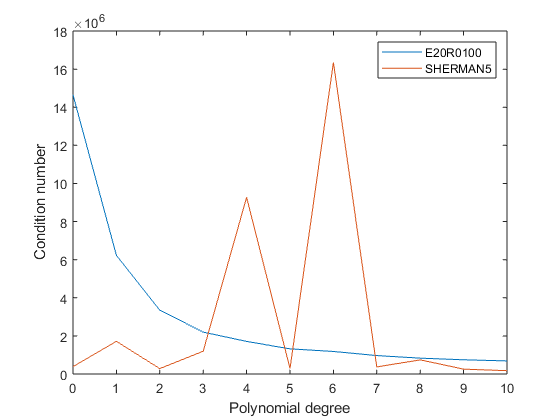
\includegraphics[width=0.45\textwidth]{example_6_condition}
\par\end{centering}
\caption{Condition numbers for E20R0100 (blue) and SHERMAN5 (orange), depending
on the polynomial degree of the preconditioner.\label{fig:cond_circle_evm}}
\end{figure}

\begin{figure}[tb]
\begin{centering}
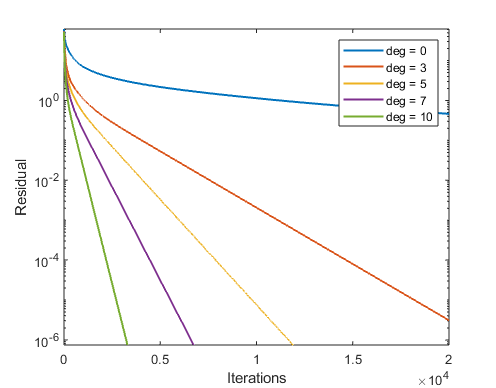
\includegraphics[width=0.4\textwidth]{example_4_gmres}
\par\end{centering}
\caption{Convergence of S1RMQ4M1, GMRES(50) \label{fig:convergence_s1rmq4m1}}
\end{figure}

\begin{figure}[tb]
\begin{centering}
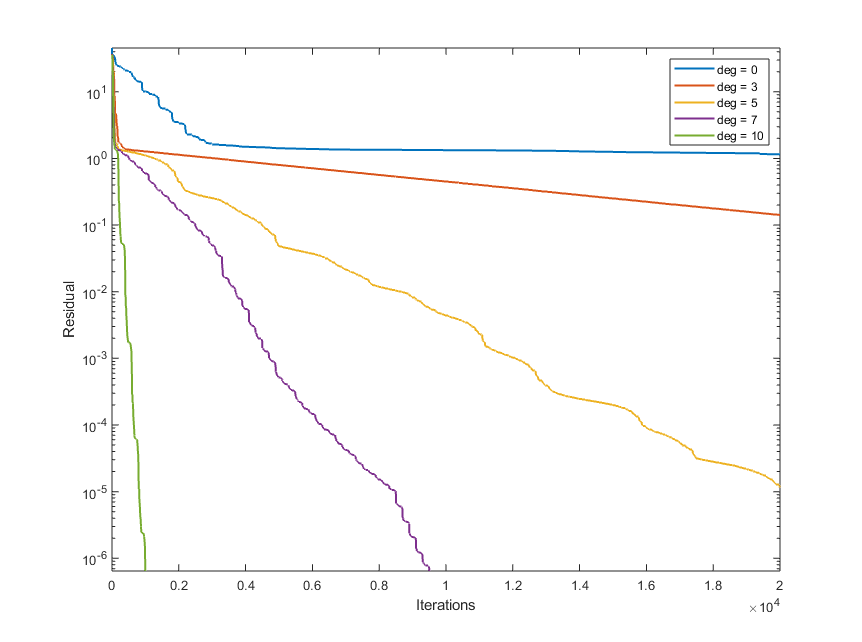
\includegraphics[width=0.4\textwidth]{example_5_gmres}
\par\end{centering}
\caption{Convergence of E20R0100, GMRES(100) \label{fig:convergence_e20r0100}}
\end{figure}

\begin{figure}[t]
\begin{centering}
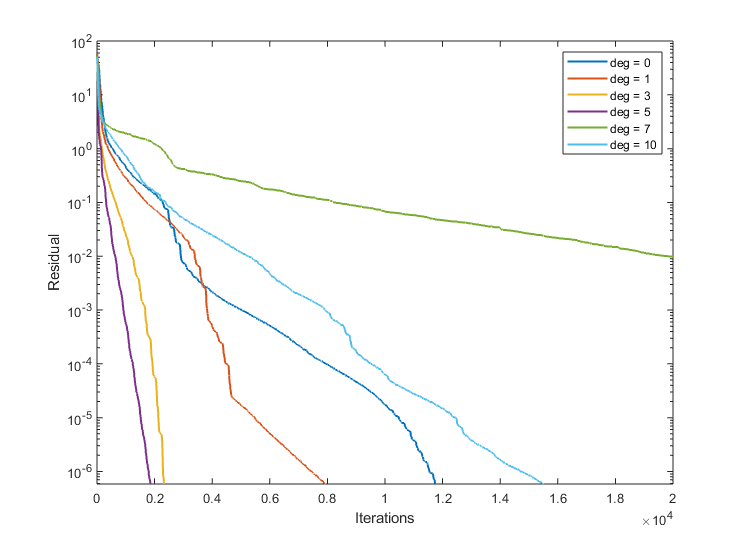
\includegraphics[width=0.4\textwidth]{example_6_gmres_seed_42}
\par\end{centering}
\caption{Convergence of SHERMAN5, GMRES(100), seed = 42 \label{fig:convergence_SHERMAN5-1}}
\end{figure}

\begin{figure}[tb]
\begin{centering}
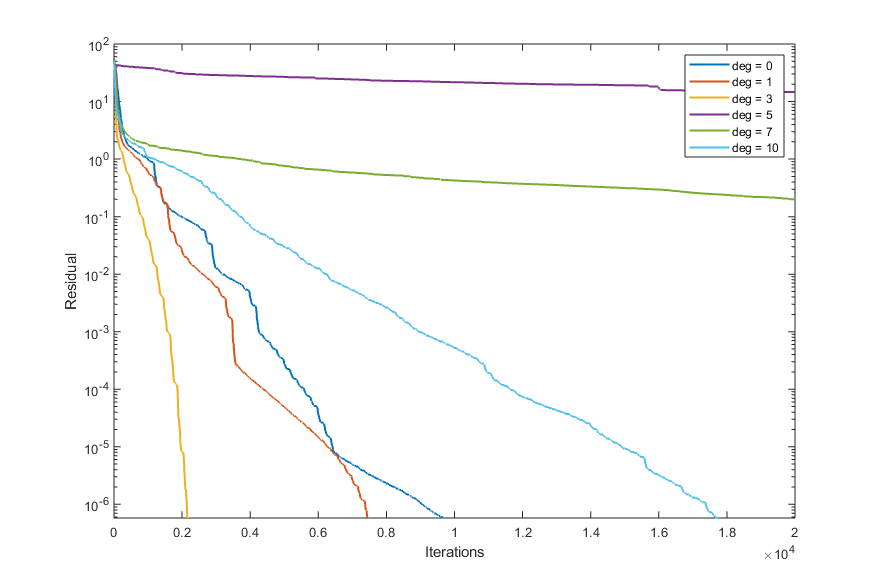
\includegraphics[width=0.39\textwidth]{example_6_gmres_seed_1892}
\par\end{centering}
\caption{Convergence of SHERMAN5, GMRES(100), seed = 1892 \label{fig:convergence_SHERMAN5-2}}
\end{figure}


\section*{Conclusion}

Polynomial preconditioners can be used along with standard preconditioning,
and are effective to implement on parallel systems as a series of
sparse matrix-vector products. We have introduced a polynomial preconditioner
related to the minimum residual (GMRES) polynomial. 

To compute the coefficient of the polynomial, no knowledge of the
spectrum of $A$ is required. It suffices to take a random vector
$v_{0}$, and solve the least squares problem $\min\|v_{0}-s(A)Av_{0}\|$.
This however bases on computing a power basis $(A^{i}v_{0})$, which
is ill-conditioned. Therefore the degree of the polynomial is limited,
typically to $d\leq10$.

Applying this preconditioner to several difficult problems, including
E20R0100, shows it can be used to significantly improve convergence
of GMRES. In particular, on parallel systems, synchronization points
from inner products in each GMRES step are reduced. 

Care should be taken for problems such as SHERMAN5, where effectiveness
varies for different samples of the vector $v_{0}$, and can even
result in worse convergence.
\begin{thebibliography}{10}
\bibitem{Saad-1986}Y. SAAD, M. H. Schultz, \emph{GMRES: A generalized
minimal residual algorithm for solving nonsymmetric linear systems,}
SIAM J. Sci. Stat. Comput. Vol. 7, No. 3, July 1986.

\bibitem{Saad-1985}Y. SAAD, \emph{Practical use of polynomial preconditionings
for the conjugate gradient method}, SIAM J. Sci. Stat. Comput. Vol.
6, No. 4, October 1985.

\bibitem{Magoules-2015}F. MAGOULES, F. ROUX, G. HOUZEAUX, \emph{Parallel
Scientific Computing, }Wiley, 2015.

\bibitem{Saad-2003}Y. SAAD, \emph{Iterative Methods for Sparse Linear
Systems}, SIAM, 2003.

\bibitem{Trefethen-1997}L. N. TREFETHEN, D. BAU, \emph{Numerical
Linear Algebra}, SIAM, 1997.

\bibitem{Benzi-2005}M. BENZI, G. H. GOLUB, J. LIESEN, \emph{Numerical
solution of saddle point problems, }Acta Numerica (2005), pp. 1-137.

\bibitem{Rozlo=00017En=0000EDk-2018}M. ROZLOŽNÍK, \emph{Saddle-Point
Problems and Their Iterative Solution}, Birkhäuser, 2018.

\bibitem{Barret-1994}R. BARRET et. al., \emph{Templates for the Solution
of Linear Sytems: Building Blocks for Iterative Methods}, SIAM, 1994.

\bibitem{Liu-2015}Q. LIU, R. B. MORGAN, W. WILCOX, \emph{Polynomial
Preconditioned GMRES and GMRES-DR}, SIAM J. Sci. Comput. Vol. 37,
No. 5, pp. S407-S428, 2015.

\bibitem{Loe-2019}J. A. LOE, H. K. THORNQUIST, E. G. BOMAN, \emph{Polynomial
Preconditioned GMRES to Reduce Communication in Parallel Computing},
arXiv, Oct 2019.

\bibitem{Hernandez-2005}V. HERNANDÉZ, J. E. ROMÁN, A. TOMAS, \emph{A
Parallel Variant of the Gram-Schmidt Process with Reorthogonalization},
Proceedings of the International Conference Parco 2005, 13-16 September
2005.
\end{thebibliography}

\end{document}
